% Aberdeen style guide should be followed when using this
% layout. Their template powerpoint slide is used to extract the
% Aberdeen color and logo but is otherwise ignored (it has little or
% no formatting in it anyway).
%
% http://www.abdn.ac.uk/documents/style-guide.pdf

%%%%%%%%%%%%%%%%%%%% Document Class Settings %%%%%%%%%%%%%%%%%%%%%%%%%
% Pick if you want slides, or draft slides (no animations)
%%%%%%%%%%%%%%%%%%%%%%%%%%%%%%%%%%%%%%%%%%%%%%%%%%%%%%%%%%%%%%%%%%%%%%
%Normal document mode%
\documentclass[10pt,compress]{beamer}
%Draft or handout mode
%\documentclass[10pt,compress,handout]{beamer}
%\documentclass[10pt,compress,handout,ignorenonframetext]{beamer}

%%%%%%%%%%%%%%%%%%%% General Document settings %%%%%%%%%%%%%%%%%%%%%%%
% These settings must be set for each presentation
%%%%%%%%%%%%%%%%%%%%%%%%%%%%%%%%%%%%%%%%%%%%%%%%%%%%%%%%%%%%%%%%%%%%%%
\newcommand{\shortname}{jefferson.gomes@abdn.ac.uk}
\newcommand{\fullname}{Dr Jeff Gomes}
\institute{School of Engineering}
\newcommand{\emailaddress}{}%jefferson.gomes@abdn.ac.uk}
\newcommand{\logoimage}{../../FigBanner/UoAHorizBanner}
\title{Chemical Thermodynamics (EX3029)}
\subtitle{Module 2: Second Law of Thermodynamics}
%\subtitle{Module 1.1: Review of Thermodynamics}
\date[ ]{ }

%%%%%%%%%%%%%%%%%%%% Template settings %%%%%%%%%%%%%%%%%%%%%%%%%%%%%%%
% You shouldn't have to change below this line, unless you want to.
%%%%%%%%%%%%%%%%%%%%%%%%%%%%%%%%%%%%%%%%%%%%%%%%%%%%%%%%%%%%%%%%%%%%%%
\usecolortheme{whale}
\useoutertheme{infolines}

% Use the fading effect for items that are covered on the current
% slide.
\beamertemplatetransparentcovered

% We abuse the author command to place all of the slide information on
% the title page.
\author[\shortname]{%
  \fullname\\\ttfamily{\emailaddress}
}


%At the start of every section, put a slide indicating the contents of the current section.
%\AtBeginSection[] {
%  \begin{frame}
%    \frametitle{Section Outline}
%    \tableofcontents[currentsection]
%  \end{frame}
%}

% Allow the inclusion of movies into the Presentation! At present,
% only the Okular program is capable of playing the movies *IN* the
% presentation.
\usepackage{multimedia}
\usepackage{animate}

%% Handsout -- comment out the lines below to create handstout with 4 slides in a page with space for comments
\usepackage{handoutWithNotes}
%\pgfpagesuselayout{2 on 1 with notes}[a4paper,border shrink=10mm]
%%%%% Color settings
\usepackage{color}
%% The background color for code listings (i.e. example programs)
\definecolor{lbcolor}{rgb}{0.9,0.9,0.9}%
\definecolor{UoARed}{rgb}{0.64706, 0.0, 0.12941}
\definecolor{UoALight}{rgb}{0.85, 0.85, 0.85}
\definecolor{UoALighter}{rgb}{0.92, 0.92, 0.92}
\setbeamercolor{structure}{fg=UoARed} % General background and higlight color
\setbeamercolor{frametitle}{bg=black} % General color
\setbeamercolor{frametitle right}{bg=black} % General color
\setbeamercolor{block body}{bg=UoALighter} % For blocks
\setbeamercolor{structure}{bg=UoALight} % For blocks
% Rounded boxes for blocks
\setbeamertemplate{blocks}[rounded]

%%%%% Font settings
% Aberdeen requires the use of Arial in slides. We can use the
% Helvetica font as its widely available like so
% \usepackage{helvet}
% \renewcommand{\familydefault}{\sfdefault}
% But beamer already uses a sans font, so we will stick with that.

% The size of the font used for the code listings.
\newcommand{\goodsize}{\fontsize{6}{7}\selectfont}

% Extra math packages, symbols and colors. If you're using Latex you
% must be using it for formatting the math!
\usepackage{amscd,amssymb} \usepackage{amsfonts}
\usepackage[mathscr]{eucal} \usepackage{mathrsfs}
\usepackage{latexsym} \usepackage{amsmath} \usepackage{bm}
\usepackage{amsthm} \usepackage{textcomp} \usepackage{eurosym}
% This package provides \cancel{a} and \cancelto{a}{b} to "cancel"
% expressions in math.
\usepackage{cancel}

\usepackage{comment} 

% Get rid of font warnings as modern LaTaX installations have scalable
% fonts
\usepackage{type1cm} 

%\usepackage{enumitem} % continuous numbering throughout enumerate commands

% For exact placement of images/text on the cover page
\usepackage[absolute]{textpos}
\setlength{\TPHorizModule}{1mm}%sets the textpos unit
\setlength{\TPVertModule}{\TPHorizModule} 

% Source code formatting package
\usepackage{listings}%
\lstset{ backgroundcolor=\color{lbcolor}, tabsize=4,
  numberstyle=\tiny, rulecolor=, language=C++, basicstyle=\goodsize,
  upquote=true, aboveskip={1.5\baselineskip}, columns=fixed,
  showstringspaces=false, extendedchars=true, breaklines=false,
  prebreak = \raisebox{0ex}[0ex][0ex]{\ensuremath{\hookleftarrow}},
  frame=single, showtabs=false, showspaces=false,
  showstringspaces=false, identifierstyle=\ttfamily,
  keywordstyle=\color[rgb]{0,0,1},
  commentstyle=\color[rgb]{0.133,0.545,0.133},
  stringstyle=\color[rgb]{0.627,0.126,0.941}}

% Allows the inclusion of other PDF's into the final PDF. Great for
% attaching tutorial sheets etc.
\usepackage{pdfpages}
\setbeamercolor{background canvas}{bg=}  

% Remove foot note horizontal rules, they occupy too much space on the slide
\renewcommand{\footnoterule}{}

% Force the driver to fix the colors on PDF's which include mixed
% colorspaces and transparency.
\pdfpageattr {/Group << /S /Transparency /I true /CS /DeviceRGB>>}

% Include a graphics, reserve space for it but
% show it on the next frame.
% Parameters:
% #1 Which slide you want it on
% #2 Previous slides
% #3 Options to \includegraphics (optional)
% #4 Name of graphic
\newcommand{\reserveandshow}[4]{%
\phantom{\includegraphics<#2|handout:0>[#3]{#4}}%
\includegraphics<#1>[#3]{#4}%
}

\begin{document}

% Title page layout
\begin{frame}
  \titlepage
  \vfill%
  \begin{center}
    \includegraphics[clip,width=0.8\textwidth]{\logoimage}
  \end{center}
\end{frame}

% Table of contents
%\frame{ \frametitle{Slides Outline}
%  \tableofcontents
%}


%%%%%%%%%%%%%%%%%%%% The Presentation Proper %%%%%%%%%%%%%%%%%%%%%%%%%
% Fill below this line with \begin{frame} commands! It's best to
% always add the fragile option incase you're going to use the
% verbatim environment.
%%%%%%%%%%%%%%%%%%%%%%%%%%%%%%%%%%%%%%%%%%%%%%%%%%%%%%%%%%%%%%%%%%%%%%



%%%
%%% SECTION
%%%
\section{General Remarks}

%%%
%%% Slides
%%%
\begin{frame}
 \frametitle{Aims and Objectives}
   \begin{enumerate}
     \item<1-> In Module 1, we learnt:
       \begin{enumerate}
         \item<1-> \textcolor{blue}{Zeroth Law:} Bodies are in thermal equilibrium if they are at the same temperature.
         \item<1-> \textcolor{blue}{First Law:} Energy is conserved during a process.
       \end{enumerate} 
     \item<2-> However, the Fist Law is not able to help either 
       \begin{enumerate}
         \item<2-> clarifying the natural direction of a process (\textcolor{blue}{reversibility}) or;
         \item<2-> to assess the efficiency of a thermal process.
       \end{enumerate}
     \item<3-> In this Module, we will study the mathematical formulation of the Second Law and the definition of thermodynamic property \textcolor{blue}{\it entropy}.
   \end{enumerate}

\end{frame}

%%%
%%% SECTION
%%%
\section{Bibliography}
\begin{frame}
 \frametitle{Suggested References}
  Literature relevant for this module:
  \begin{enumerate}[(a)]
   \item J.M. Smith, H.C. Van Ness, M.M. Abbott, $\lq$Introduction to Chemical Engineering Thermodynamics', 6$^{th}$ Edition: Chapter 5;
   \item H. Devoe, $\lq$Thermodynamics and Chemistry', 2$^{nd}$ Edition: Chapter 4;
   \item M.J. Moran, H.N. Saphiro, D.D. Boettner, M.B. Bailey, $\lq$Principles of Engineering Thermodynamics', 7$^{th}$ Edition: Chapters 5 and 6.
  \end{enumerate}
\end{frame}


%%%
%%% SECTION
%%%
\section{Second Law of Thermodynamics} 

\subsection{Reversible Processes}
%%%
%%% Slides
%%%
\begin{frame}
 \frametitle{Reversible Processes}
   \begin{enumerate}
     \item<1-> In Module 01, we saw that heat is $\lq$spontaneously' transferred from a hot reservoir to a cold reservoir leading to the concept of \textcolor{blue}{reversibility}.
     \item<2-> We should remember that,
       \begin{enumerate}
         \item<2-> \textcolor{blue}{Reversible process:} A process in which it is possible to return both the system and surroundings to their original states;
         \item<3-> \textcolor{blue}{Irreversible process:} A process in which it is impossible to return both the system and surroundings to their original states.
       \end{enumerate}
    \end{enumerate}
    \begin{figure}%
     \begin{center}
      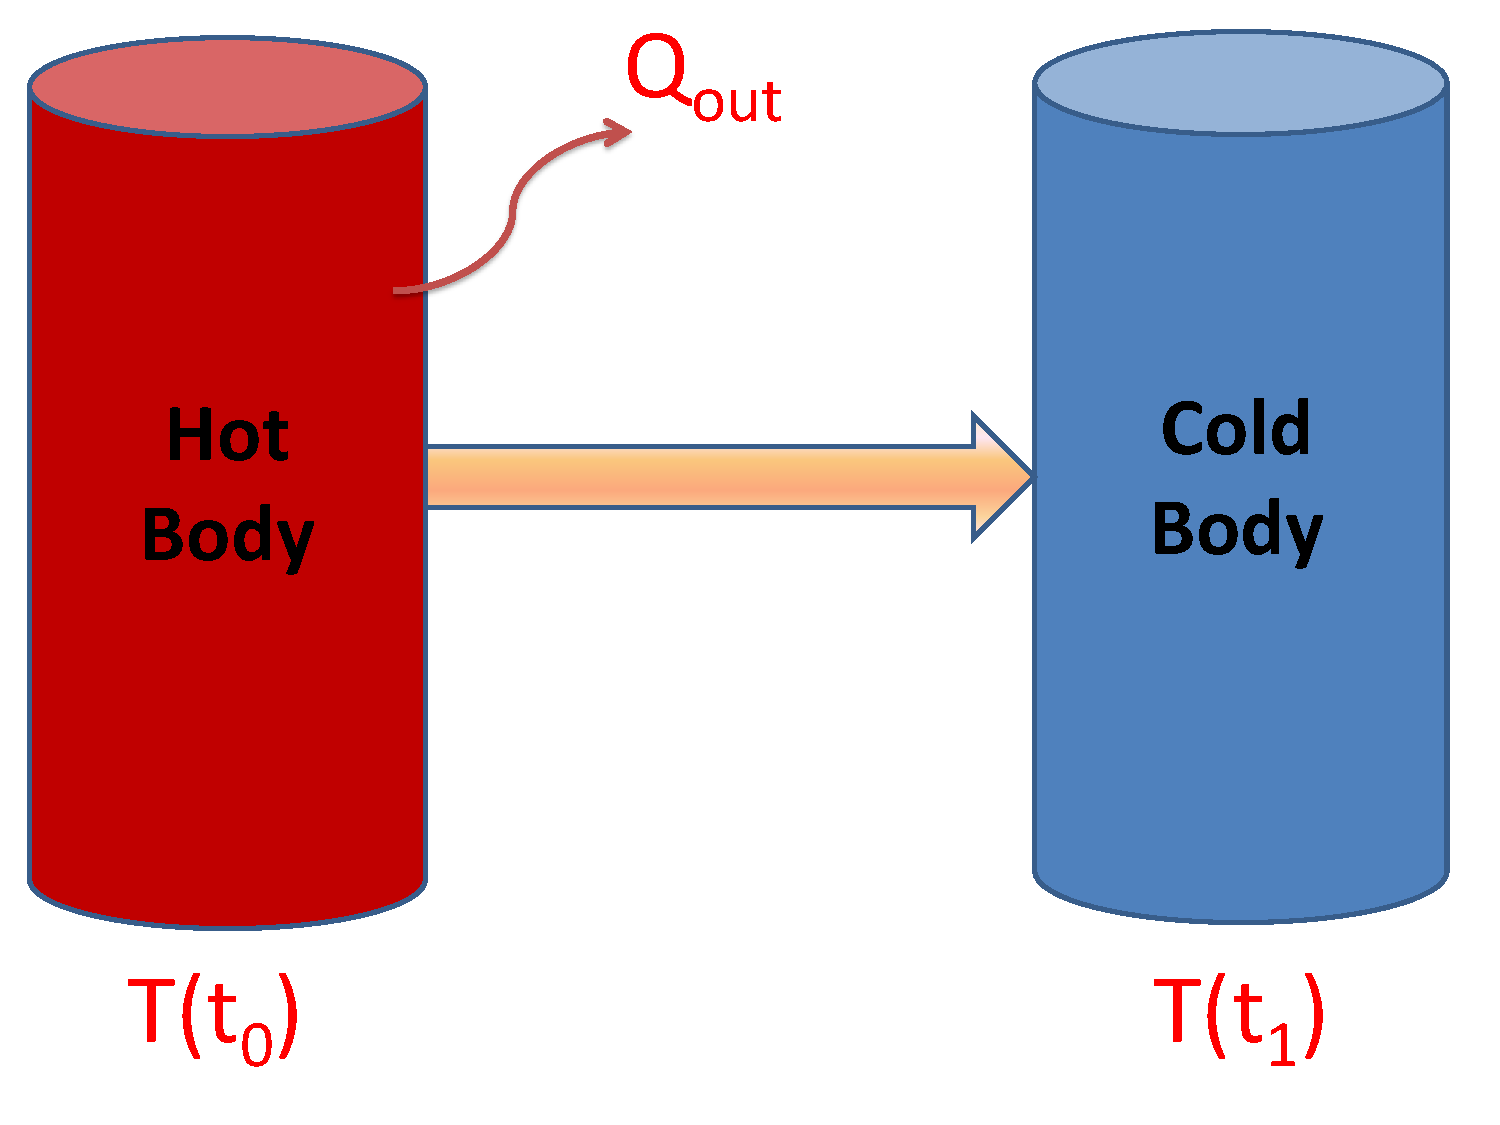
\includegraphics[width=5.5cm,clip]{./Pics/HotColdCoffee}
     \end{center}
    \end{figure}

\end{frame}

%%%
%%%  SUBSECTION
%%%
\subsection{Statements of the Second Law}

%%%
%%% Slides
%%%
\begin{frame}
 \frametitle{Second Law of Thermodynamics}
 %\scriptsize
 \begin{itemize}
   \item <2->The second law of thermodynamics is an expression of the tendency that over time, differences in temperature, pressure and chemical potential will reach an equilibrium state in an isolated physical system;
   \item <3->From the state of thermodynamic equilibrium, the law deduced the principle of the increase of entropy and explains the phenomenon of irreversibility.
 \end{itemize}

 \visible<4->{\begin{block}{R. Clausius  (1854)}
  \begin{center}
  \textcolor{blue}{$\lq$It is impossible to devise an engine which, working in a cycle, shall produce no effect other than the transfer of heat from a colder to hotter body.'}
  \end{center}
 \end{block}}

 \visible<5->{\begin{block}{Kelvin (1951) and Planck (1897)}
  \begin{center}
  \textcolor{blue}{$\lq$It is impossible to devise an engine which, working in a cycle, shall produce no effect other than the extraction of heat from a reservoir and the performance of an equal amount of mechanical work.'}
  \end{center}
 \end{block}}

 \normalsize
\end{frame}


%%%
%%% Slides
%%%
\begin{frame}
 \frametitle{Second Law of Thermodynamics}
 
   \begin{figure}%
    \begin{center}
     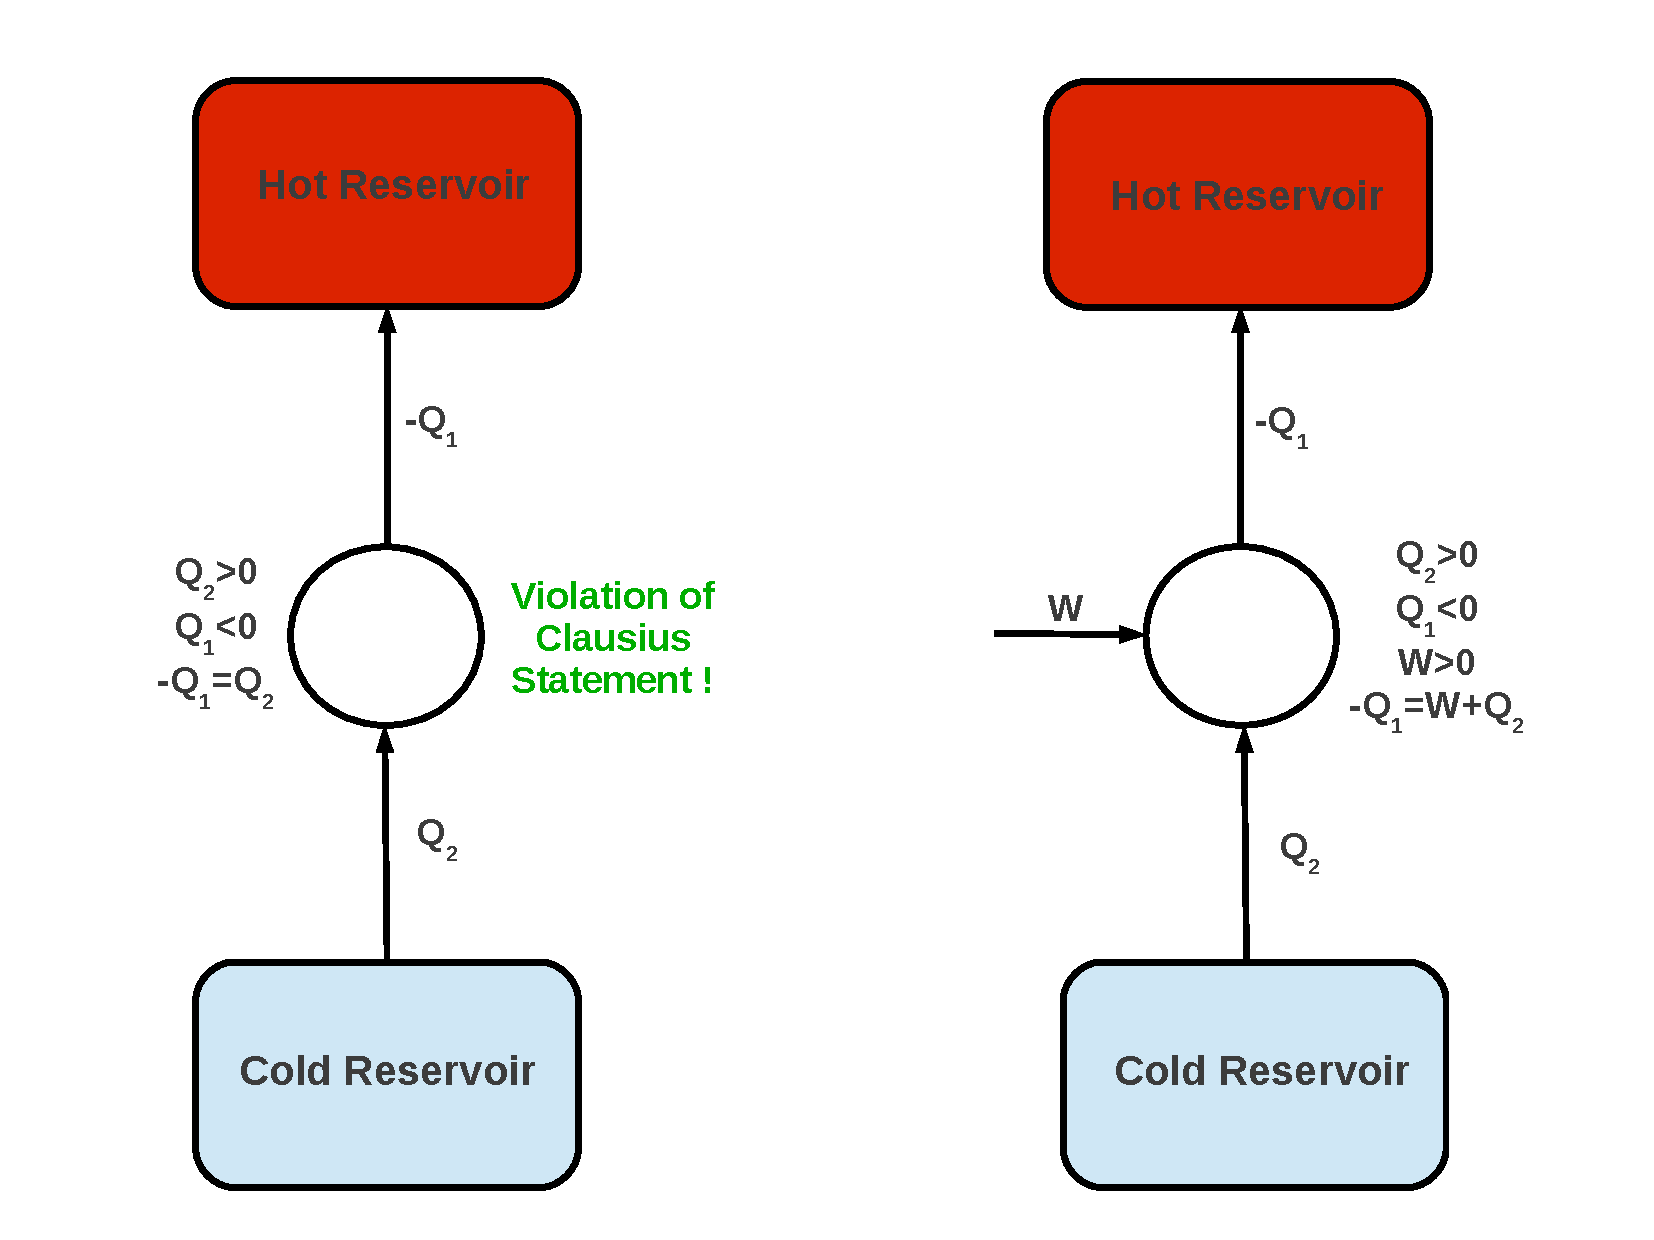
\includegraphics[width=8.cm,clip]{./Pics/2ndLaw_Schem}
    \end{center}
   \end{figure} 

   \begin{center}
     All spontaneous processes are irreversible -- heat flows from hot to cold spontaneously and irreversibly.
   \end{center}
   
\end{frame}

%%%
%%% SUBSECTION
%%%
\subsection{Second Law and Entropy}
%%%
%%% Slides
%%%
\begin{frame}
 \frametitle{Derivation of the Mathematical Statement of the Second Law}
 %\scriptsize
 \begin{columns}

  \begin{column}[c]{0.5\linewidth}
   \begin{itemize}
    \item <2-> In the schematics (rhs), an infinitesimal amount of heat, $\delta Q^{\prime}$, is transferred from the thermal reservoir (with temperature $T_{res}$) to a reversible cyclic engine (1). 
    \item <3-> The engine produces a small amount of work, $\delta W^{\prime}$, and releases an infinitesimal amount of heat, $\delta Q$ to another reservoir at variable temperature $T$. 
    \item <4-> The second reservoir (2) also releases work $\left(\delta W\right)$ to the surroundings.
   \end{itemize}


  \end{column}

  \begin{column}[c]{0.5\linewidth}
   \begin{figure}%
    \begin{center}
     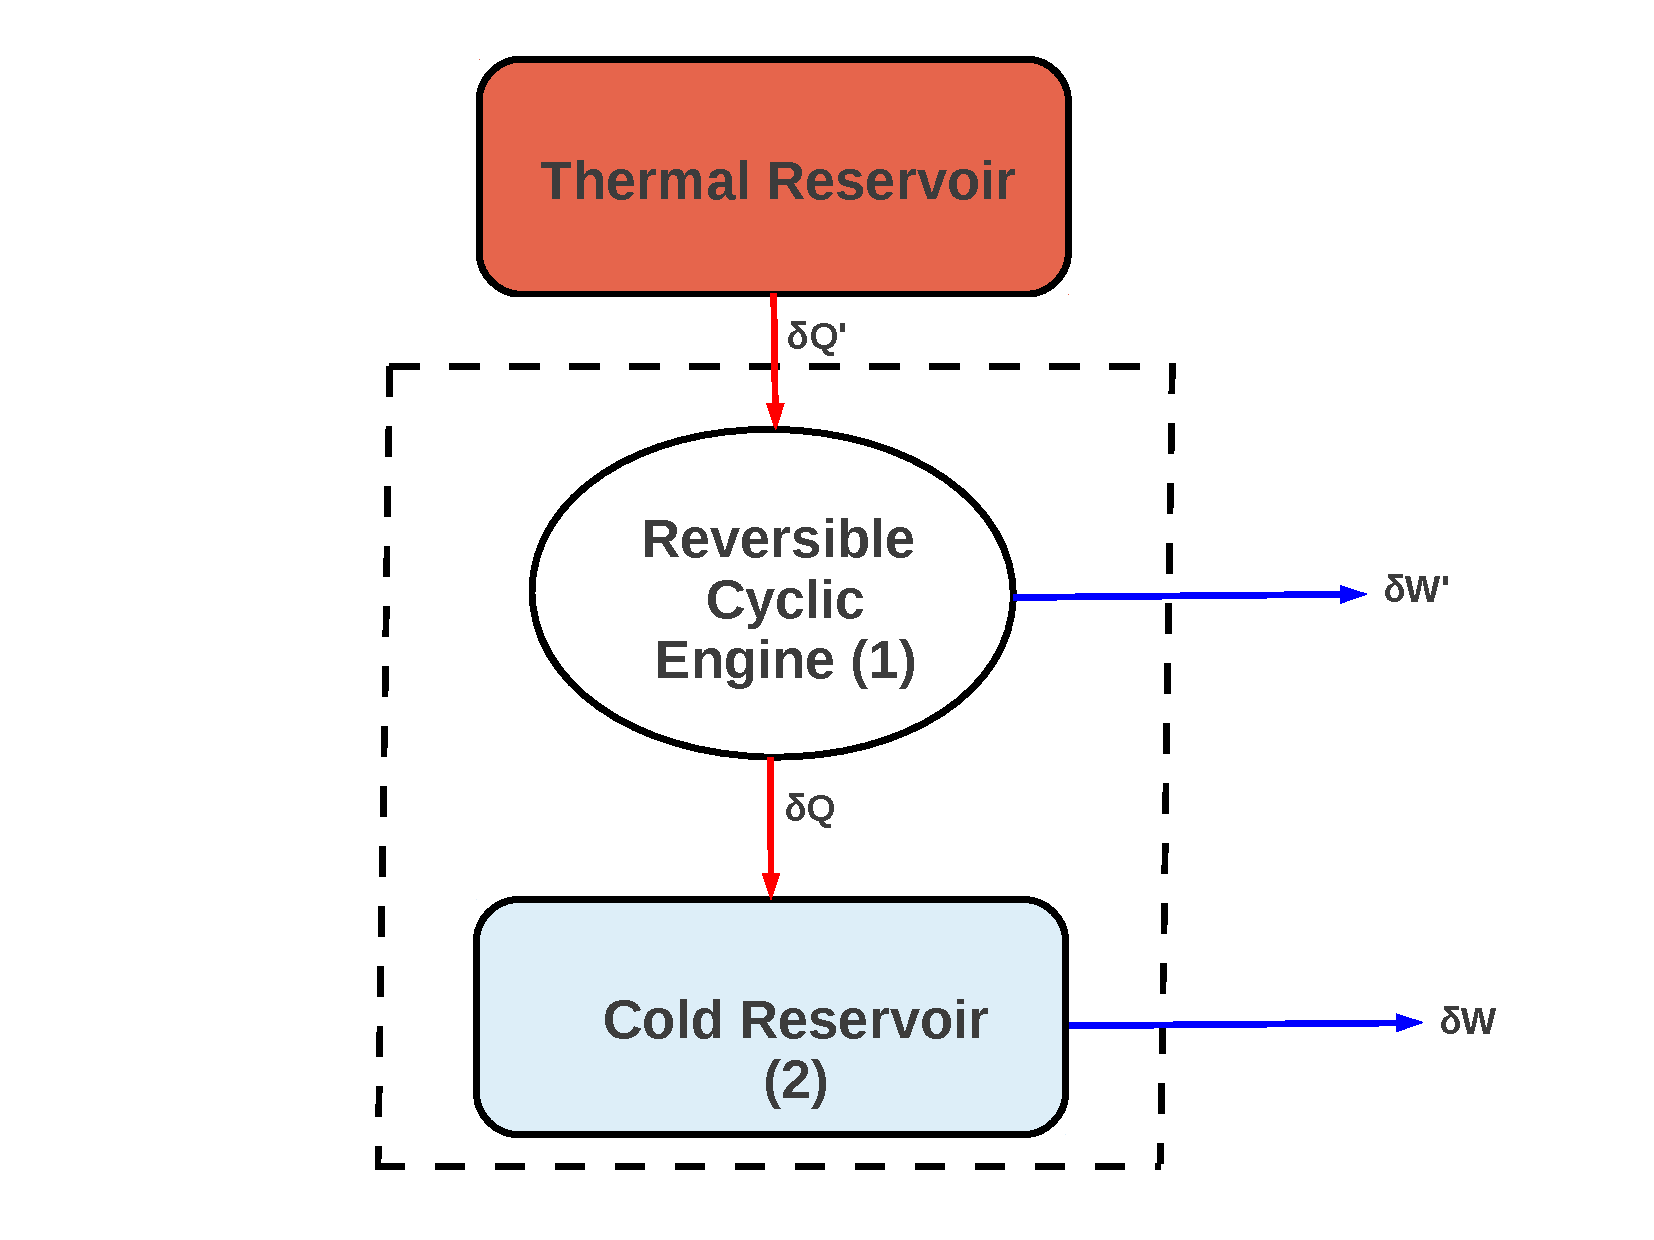
\includegraphics[width=1.1\columnwidth,clip]{./Pics/2ndLaw_Schem2}
    \end{center}
   \end{figure} 
  \end{column}
 \end{columns}


 \normalsize
    
\end{frame}

%%%
%%% Slides
%%%
\begin{frame}
 \frametitle{Derivation of the Mathematical Statement of the Second Law}
 %\scriptsize
 \begin{columns}

  \begin{column}[c]{0.5\linewidth}
   \begin{itemize}
    \item <1-> Using the analogy of heat transfer ratio and temperature ratio (see power cycle systems), \\
                $\displaystyle\frac{\delta Q^{\prime}}{\delta Q} = \displaystyle\frac{T_{res}}{T} \;\; \Longrightarrow \displaystyle\frac{\delta Q^{\prime}}{T_{res}} = \displaystyle\frac{\delta Q}{T}$
  \item <2-> The first law in differential form for the combined cycle (within the dotted box) is \\
                $dU= \delta Q^{\prime} - \left(\delta W + \delta W^{\prime}\right) \Longrightarrow \delta W + \delta W^{\prime} = \delta Q^{\prime} - dU$
  \item <3-> The process is not required to be cyclic and the heat transfer $\delta Q$ is internal and do not cross the boundary of the combined system;
   \end{itemize}


  \end{column}

  \begin{column}[c]{0.5\linewidth}
   \begin{figure}%
    \begin{center}
     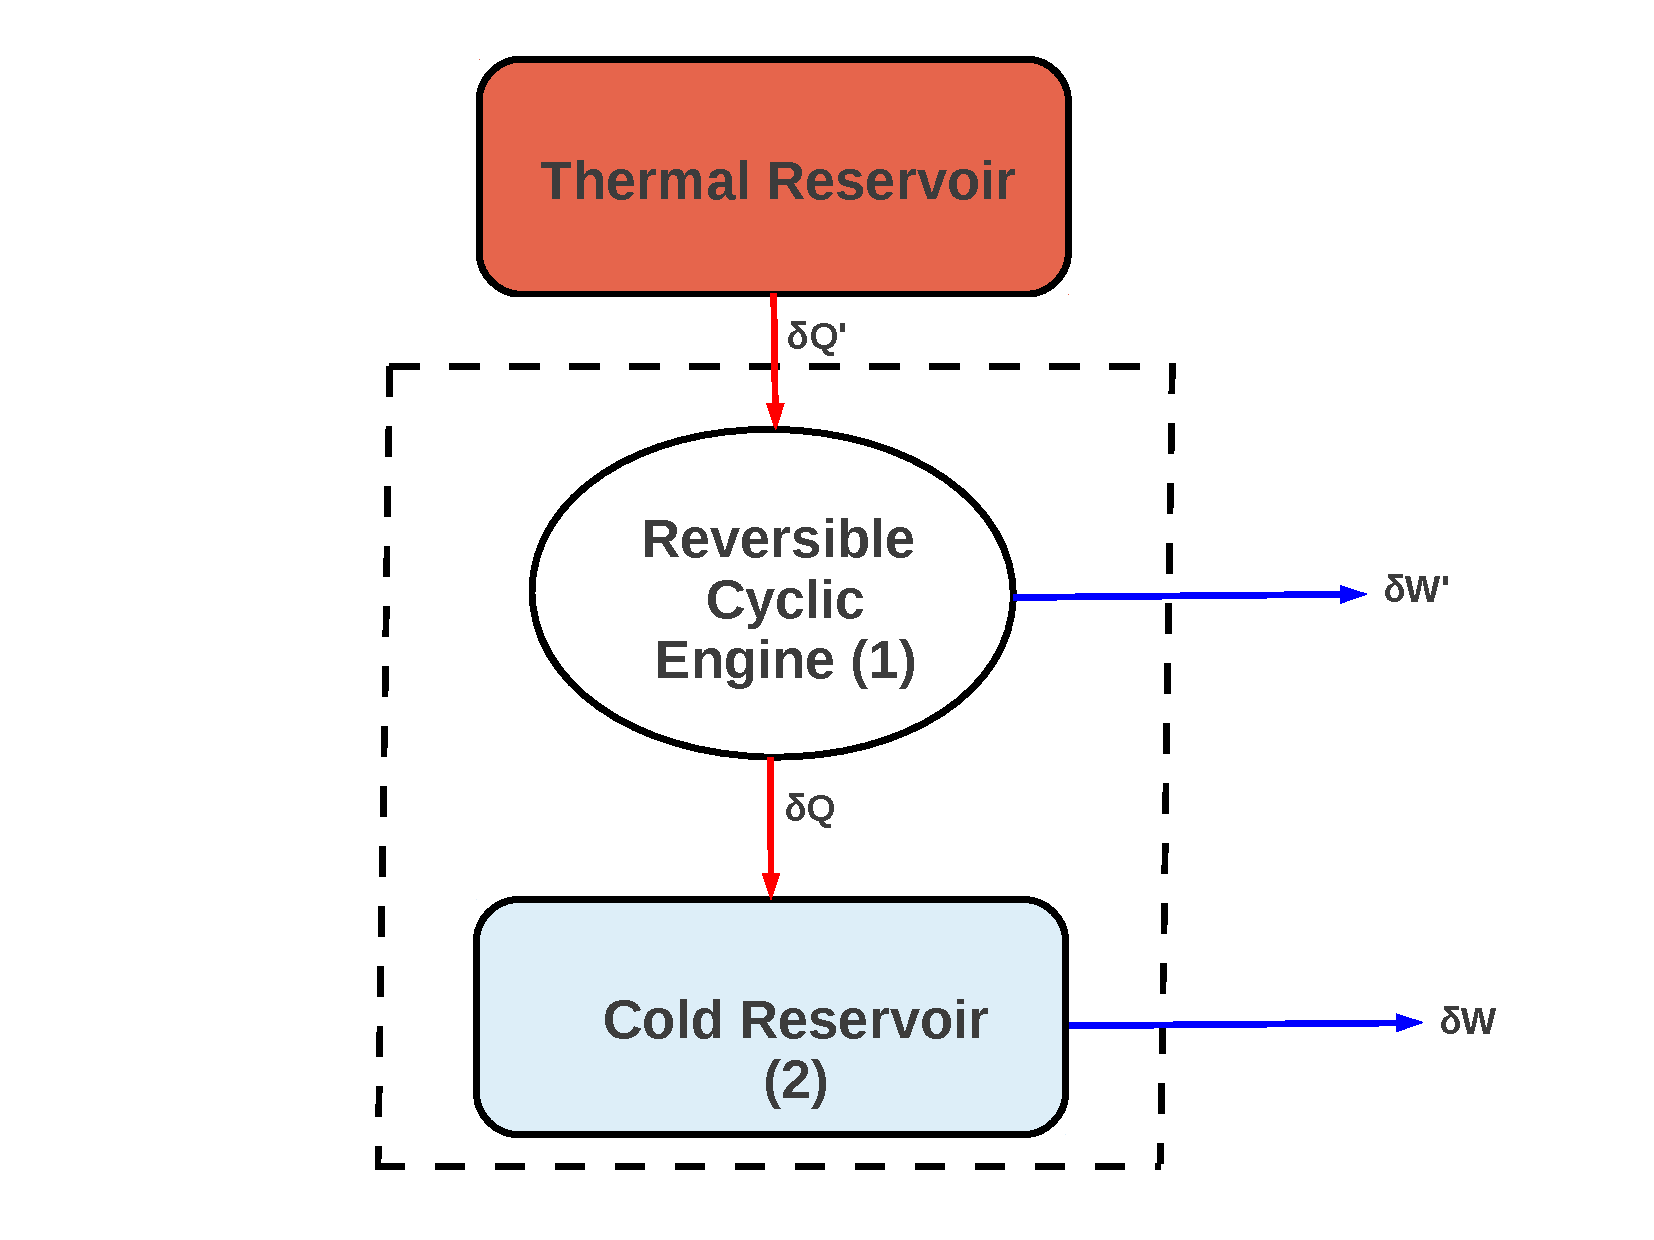
\includegraphics[width=1.1\columnwidth,clip]{./Pics/2ndLaw_Schem2}
    \end{center}
   \end{figure} 
  \end{column}
 \end{columns}


 \normalsize
    
\end{frame}


%%%
%%% Slides
%%%
\begin{frame}
 \frametitle{Derivation of the Mathematical Statement of the Second Law}
 %\scriptsize
 \begin{columns}

  \begin{column}[c]{0.5\linewidth}
   \begin{itemize}
    \item <1-> And eliminating $\delta Q^{\prime}$, \\
                $\delta W + \delta W^{\prime} = T_{res}\displaystyle\frac{\delta Q}{T} - dU$
     \item <2-> If the configuration shown in the previous slide undergoes a cyclic process, \\
             $\displaystyle\oint \delta W + \displaystyle\oint \delta W^{\prime} = \displaystyle\oint T_{res}\displaystyle\frac{\delta Q}{T} - \displaystyle\oint dU$
     \item <3-> as $U$ is a thermodynamic property, the cyclic integral is equal to zero.  Integrating the equation above, and assuming that $T_{res}$ is (by definition) constant:\\
             $W + W^{\prime} = T_{res} \displaystyle\oint \displaystyle\frac{\delta Q}{T}$
   \end{itemize}
  \end{column}

  \begin{column}[c]{0.5\linewidth}
   \begin{figure}%
    \begin{center}
     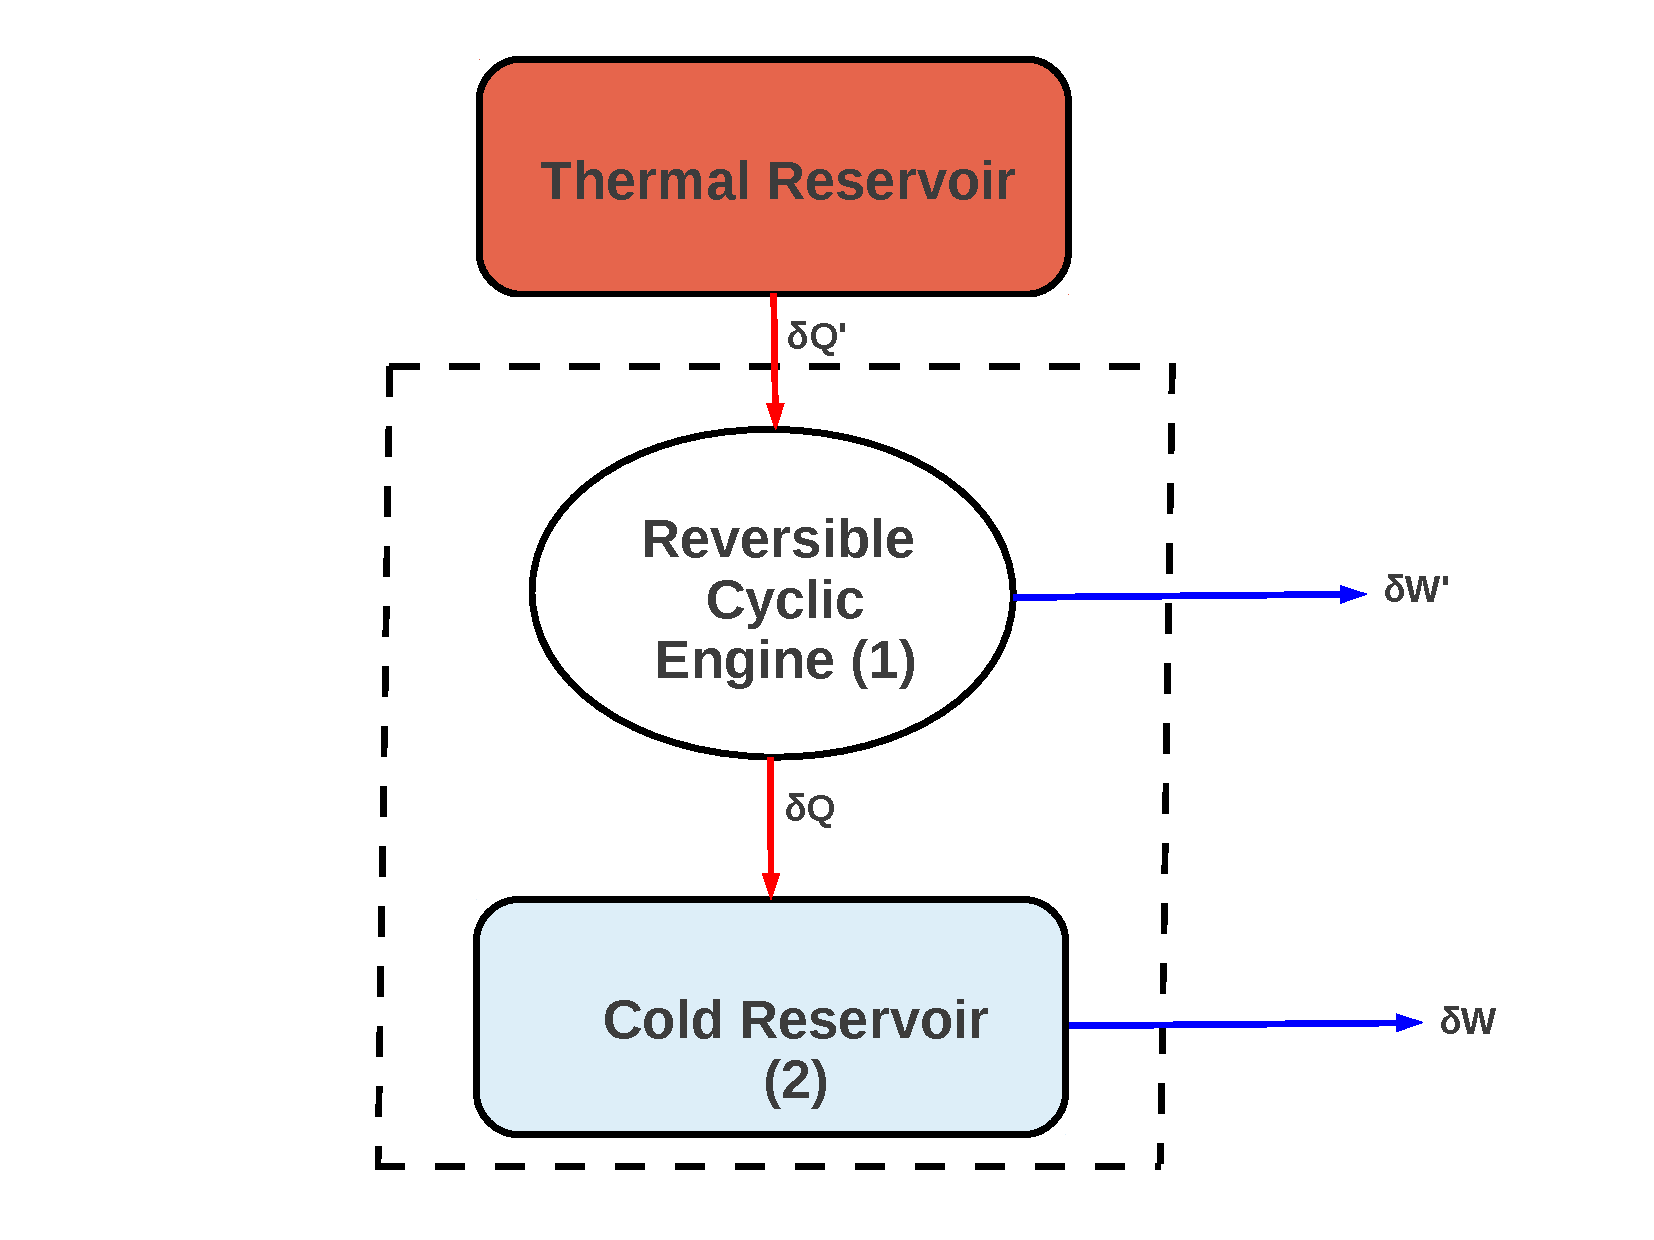
\includegraphics[width=1.1\columnwidth,clip]{./Pics/2ndLaw_Schem2}
    \end{center}
   \end{figure} 
  \end{column}
 \end{columns}
 \normalsize
    
\end{frame}


%%%
%%% Slides
%%%
\begin{frame}
 \frametitle{Derivation of the Mathematical Statement of the Second Law}
   \begin{itemize}
    \item <1-> Thus from Kelvin-Plancks statement of the Second Law -- \textcolor{blue}{$\lq$we cannot convert all the heat to work, but we can convert all the work to heat'}:\\
             $W + W^{\prime} \leq 0$
    \item <2-> And therefore,\\
             $T_{res} \displaystyle\displaystyle\oint \displaystyle\frac{\delta Q}{T} \leq 0$
    \item <3->  Since $T_{res} > 0$, we can divide the previous equation without changing the meaning of the inequality to obtain the mathematical representation of the Second Law:
             \begin{eqnarray}
             \textcolor{blue}{\displaystyle\oint \displaystyle\frac{\delta Q}{T} < 0 \;\;\; \text{for irreversible processes}} \nonumber \\
             \textcolor{blue}{\displaystyle\oint \displaystyle\frac{\delta Q}{T} = 0 \;\;\;\;\; \text{for reversible processes}} \nonumber 
             \end{eqnarray}
   \end{itemize}
 \normalsize
\end{frame}


%%%
%%% Slides
%%%
\begin{frame}
 \frametitle{Derivation of the Mathematical Statement of the Second Law}
   \begin{itemize}
    \item <1-> In a reversible process, from state 1 to 2, via path {\it A}, and returning to state 2 from either path {\it B} or {\it C}. The cyclic integral $\displaystyle\oint\displaystyle\frac{\delta Q}{T} = 0$ can be split as,
         \textcolor{blue}{\begin{eqnarray}
          \left( \displaystyle\int\limits_{1}^{2} \displaystyle\frac{\delta Q}{T} \right)_{A} + \left( \displaystyle\int\limits_{2}^{1} \displaystyle\frac{\delta Q}{T} \right)_{B} = 0 \nonumber \\
          \left( \displaystyle\int\limits_{1}^{2} \displaystyle\frac{\delta Q}{T} \right)_{A} + \left( \displaystyle\int\limits_{2}^{1} \displaystyle\frac{\delta Q}{T} \right)_{C} = 0 \nonumber 
         \end{eqnarray}}
   \end{itemize}
 \normalsize
    
\end{frame}

%%%
%%% Slides
%%%
\begin{frame}
 \frametitle{Derivation of the Mathematical Statement of the Second Law}
   \begin{itemize}
    \item <2-> Leading to:
          $\left( \displaystyle\int\limits_{1}^{2} \displaystyle\frac{\delta Q}{T} \right)_{B} = \left( \displaystyle\int\limits_{2}^{1} \displaystyle\frac{\delta Q}{T} \right)_{C} $
    \item <3-> Since paths {\it B} and {\it C} are different and arbitrary, but $\displaystyle\int\limits_{1}^{2}\displaystyle\frac{\delta Q}{T}$ is the same on either paths -- therefore \textcolor{blue}{the integral is path-independent};
    \item <4-> This defines another (extensive) thermodynamic property -- \textcolor{red}{entropy (S)}, \\
          $S_{2} - S_{1} = \displaystyle\int\limits_{1}^{2}\displaystyle\frac{\delta Q}{T}$
    \item <5-> Assuming constant mass ($m$), the intensive property entropy $\left(s=S/m\right)$, the differential form is, \\
          $ds = \displaystyle\frac{\delta q}{T} \;\;\;\; \Longrightarrow \;\;\;\; \delta q = Tds$
    \item <6-> Integrating from state 1 to 2: $q_{1}^{2} = \displaystyle\int_{1}^{2} Tds$    
   \end{itemize}
 \normalsize
\end{frame}


%%%
%%% Slides
%%%
\begin{frame}
 \frametitle{Derivation of the Mathematical Statement of the Second Law}
   \begin{itemize}
  \item <1-> This is the heat transfer equivalent of $w_{1}^{2}=\displaystyle\int_{1}^{2}PdV$
  \item <2-> Thus for a reversible process, \\
       $S_{2} - S_{1} = \displaystyle\int\limits_{1}^{2}\displaystyle\frac{\delta Q}{T}$ and $S_{1} - S_{2} = \displaystyle\int\limits_{2}^{1}\displaystyle\frac{\delta Q}{T}$;
  \item <3-> From the Second Law, \\
       $0 \geq \left( \displaystyle\int\limits_{1}^{2}\displaystyle\frac{\delta Q}{T} \right)_{A} + \left( \displaystyle\int\limits_{2}^{1}\displaystyle\frac{\delta Q}{T} \right)_{B}$ 
  \item <4-> Combinig the equations above to eliminate the path {\it B}, \\
        $S_{2}-S_{1} \geq \displaystyle\int\limits_{1}^{2}\displaystyle\frac{\delta Q}{T}$
 \end{itemize}
 \normalsize
\end{frame}




%%%
%%% Slides
%%%
\begin{frame}
 \frametitle{Derivation of the Mathematical Statement of the Second Law}
   \begin{itemize}
  \item <1-> If path {\it A} is reversible, the equality holds, however if {\it A} is irreversible, the inequality holds;
  \item <2-> If the system is isolated $\left(\delta Q = 0\right)$ then\\
    $S_{2}-S_{1}\geq 0$
   \end{itemize}
 \normalsize
    
\end{frame}


%%%
%%% SUBSECTION
%%%
\subsection{Entropy} 

%%%
%%% Slides
%%%
\begin{frame}
 \frametitle{Ideal Gas}
   \begin{enumerate}
     \item<1-> Mechanically reversible process of closed system
        \visible<1->{\begin{displaymath}
           dU = dQ_{\text{rev}} - PdV
        \end{displaymath}}
     \item<2-> Applying the definition of entropy and enthalpy,
        \visible<2->{\begin{displaymath}
           \displaystyle\frac{\Delta S}{R} = \int\limits_{T_{0}}^{T}\displaystyle\frac{C_{p}^{\text{ig}}}{R}\displaystyle\frac{d T}{T} - \ln\displaystyle\frac{P}{P_{0}}
        \end{displaymath}}
     \item<2-> This relates {\bf only} to \textcolor{blue}{properties}, i.e., \textcolor{blue}{independent of the process}.
   \end{enumerate}
 \normalsize
\end{frame}


\subsection{Summary}
%%%
%%% Slides
%%%
\begin{frame}
 \frametitle{Summary}
After this Module you should know: 
 \begin{itemize}
  \item <1-> Reversibility and its impact on thermodynamics formulation;
  \item <2-> Statements of the Second law and applications;
  \item <3-> Definition of entropy.
 \end{itemize}
\end{frame}

\end{document}
